%% LyX 1.5.3 created this file.  For more info, see http://www.lyx.org/.
%% Do not edit unless you really know what you are doing.
\documentclass[english]{beamer}
\usepackage[latin9]{inputenc}
\usepackage{subfigure}
\usepackage{color}
\usepackage{graphicx}
\usepackage{amssymb,amsmath}
\usepackage[authoryear]{natbib}

\makeatletter

%%%%%%%%%%%%%%%%%%%%%%%%%%%%%% LyX specific LaTeX commands.
%% Because html converters don't know tabularnewline
\providecommand{\tabularnewline}{\\}
%% A simple dot to overcome graphicx limitations
\newcommand{\lyxdot}{.}


%%%%%%%%%%%%%%%%%%%%%%%%%%%%%% Textclass specific LaTeX commands.
 \AtBeginDocument{
   \let\origtableofcontents=\tableofcontents
   \def\tableofcontents{\@ifnextchar[{\origtableofcontents}{\gobbletableofcontents}}
   \def\gobbletableofcontents#1{\origtableofcontents}
 }
 \makeatletter
 \long\def\lyxframe#1{\@lyxframe#1\@lyxframestop}%
 \def\@lyxframe{\@ifnextchar<{\@@lyxframe}{\@@lyxframe<*>}}%
 \def\@@lyxframe<#1>{\@ifnextchar[{\@@@lyxframe<#1>}{\@@@lyxframe<#1>[]}}
 \def\@@@lyxframe<#1>[{\@ifnextchar<{\@@@@@lyxframe<#1>[}{\@@@@lyxframe<#1>[<*>][}}
 \def\@@@@@lyxframe<#1>[#2]{\@ifnextchar[{\@@@@lyxframe<#1>[#2]}{\@@@@lyxframe<#1>[#2][]}}
 \long\def\@@@@lyxframe<#1>[#2][#3]#4\@lyxframestop#5\lyxframeend{%
   \frame<#1>[#2][#3]{\frametitle{#4}#5}}
 \makeatother
 \newenvironment{centercolumns}{\begin{columns}[c]}{\end{columns}}
 \def\lyxframeend{} % In case there is a superfluous frame end

%%%%%%%%%%%%%%%%%%%%%%%%%%%%%% User specified LaTeX commands.
 \setbeamercovered{transparent}
\usepackage{listings}

\setbeamertemplate{navigation symbols}{} 
%\useoutertheme{infolines} 
% \usecolortheme{tkk}
%\usetheme{Warsaw}
% or ...
%\usetheme{Antibes}	% tree outline, neat
%\usetheme{JuanLesPins}	% like Antibes, with shading
%\usetheme{Bergen}	% outline on side
%\usetheme{Luebeck}	% like Warsaw, square sides
%\usetheme{Berkeley}	% interesting left bar outline
%\usetheme{Madrid}	% clean, nice.  7/12 page numbers
%\usetheme{Berlin}	% dots show slide number
%\usetheme{Malmoe}	% OK, plain, unshaded
% \usetheme{Boadilla}	% nice, white bg, no top bar
%\usetheme{Marburg}	% nice, outline on right
%\usetheme{boxes}	% ???
%\usetheme{Montpellier}	% tree outline on top, plainish white
%\usetheme{Copenhagen}	% like Warsaw
%\usetheme{PaloAlto}	% looks good
%\usetheme{Darmstadt}	% like Warsaw with circle outline
\usetheme{Pittsburgh}
%\usetheme{default}
%\usetheme{Rochester}	% like boxy, unshaded warsaw
%\usetheme{Dresden}	% circle outline on top
%\usetheme{Singapore}	% purple gradient top
%\usetheme{Frankfurt}	% like Warsaw with circle outline on top
%\usetheme{Szeged}
%\usetheme{Goettingen}	% light purple right bar outline
%\usetheme{Warsaw}
%\usetheme{Hannover}	% like Goett with bar on left
%\usetheme{compatibility}
%\usetheme{Ilmenau}

\setbeamercovered{transparent}
% or whatever (possibly just delete it)

%\usecolortheme{seahorse}
%\usecolortheme{rose}

% seems to fix typewriter font in outline header:
\usepackage{ae,aecompl}

\newcommand{\newblock}{}
\newcommand{\mymathrm}[1]{\mathrm{#1}}

\definecolor{DRed}{rgb}{0.8,0.6,0.6}
\definecolor{DGreen}{rgb}{0.6,0.7,0.6}
\definecolor{DBlue}{rgb}{0.6,0.6,0.8}
\definecolor{DYellow}{rgb}{0.8,0.8,0.6}
\definecolor{Yellow}{rgb}{1,1,0.8}
\definecolor{Cream}{rgb}{1,1,1}
\definecolor{White}{rgb}{1,1,1}
\definecolor{Black}{rgb}{0,0,0}
\definecolor{BRed}{rgb}{0.6,0,0}
\definecolor{BGreen}{rgb}{0,0.6,0}
\definecolor{BBlue}{rgb}{0,0,0.6}
\definecolor{darkblue}{rgb}{0.0,0.1,0.4}
\definecolor{LGrey}{rgb}{0.6,0.6,0.6}
\definecolor{LRed}{rgb}{0.8,0.5,0.5}
\definecolor{LGreen}{rgb}{0.5,0.8,0.5}
\definecolor{LBlue}{rgb}{0.5,0.5,0.8}

\newcommand{\myred}[1]{{\color{BRed}#1}}
\newcommand{\mygreen}[1]{{\color{BGreen}#1}}
\newcommand{\mylred}[1]{{\color{LRed}#1}}
\newcommand{\mylgreen}[1]{{\color{LGreen}#1}}
\newcommand{\myblue}[1]{{\color{blue}#1}}


% CVRG Dimensionality Reduction


%\mode<article>
%{
 %\usepackage{fullpage}

%  \usepackage{pgf}

%  \usepackage{hyperref}

 % \usepackage{multimedia}
%  \usepackage{url}

%  \usepackage{urlh}

%  \setjobnamebeamerversion{beamerexample2.beamer}
%}

%\mode<presentation>
%{
 %\usetheme{Singapore} % CHANGE THEME
%  \usetheme{Berkeley}  

%  \setbeamercovered{transparent}
%}





%\institute{Oxford Brookes University
%  \and University of Manchester}
\usepackage{xmpmulti}

\usepackage{bm}


%%%%%%%%%%%%%%%%%%%%%%%%%%%%%% User specified LaTeX commands.



\usepackage{subfigure}




%%%%%%%%%%%%%%%%%%%%%%%%%%%%%%%%%%%%%%%%%%%%%%%%%%%%%%%%%%%%%%%%%%%%%%%%%%%%%%%%%%%%%%%%
%%%%%%%%%%%%%%%%%%%%%%%%%%%%%%%%%%%%%%%%%%%%%%%%%%%%%%%%%%%%%%%%%%%%%%%%%%%%%%%%%%%%%%%%%

\usepackage{babel}
\makeatother

\begin{document}
\selectlanguage{english}

%\title[ML Systems Biology]{Statistical Inference in Systems Biology through Gaussian Processes
%and Ordinary Differential Equations }
\title{Transcription factor target identification with limited data using
Gaussian process models}

\author{Antti Honkela\\
  with Neil D. Lawrence, Magnus Rattray and Michalis Titsias}

\institute{Aalto University School of Science and Technology\\
  Department of Information and Computer Science}
\titlegraphic{\includegraphics[width=.5\textwidth]{Aalto_EN_ScienceandTech_13_CMYK-UNCOATED_2}\hspace*{.1\textwidth}\includegraphics[width=.2\textwidth]{manchester_logo}}

%\author[Neil D. Lawrence]{\textbf{Neil D. Lawrence} and Magnus Rattray\\
%Researchers: Pei Gao, Michalis Titsias, Antti Honkela, Jennifer Withers}


%\institute[Ringberg Castle]{Max Planck Institute, Ringberg Castle}
%\institute{Tampere University of Technology, Department of Signal Processing}


\date{11 May 2010}

\frame{\maketitle}
\newcommand{\bfdelta}{\boldsymbol{\delta}}
 \newcommand{\bfDelta}{\boldsymbol{\Delta}}
 \newcommand{\bfbeta}{\boldsymbol{\beta}}
 \newcommand{\bfgamma}{\boldsymbol{\gamma}}
 \newcommand{\bfmu}{\bm{\mu}}
 \newcommand{\bfnu}{\boldsymbol{\nu}}
 \newcommand{\bfalpha}{\boldsymbol{\alpha}}
 \newcommand{\bfepsilon}{\boldsymbol{\epsilon}}
 \newcommand{\bfSigma}{\boldsymbol{\Sigma}}
 \newcommand{\bftau}{\boldsymbol{\tau}}
 \newcommand{\bflambda}{\boldsymbol{\lambda}}
 \newcommand{\bfLambda}{\boldsymbol{\Lambda}}
 \newcommand{\bfpsi}{\boldsymbol{\psi}}
 \newcommand{\bfxi}{\boldsymbol{\xi}}
 \newcommand{\bfpi}{\bm{\pi}}
 \newcommand{\bfPsi}{\boldsymbol{\Psi}}
 \newcommand{\bfphi}{\boldsymbol{\phi}}
 \newcommand{\bfPhi}{\boldsymbol{\Phi}}
 \newcommand{\bfrho}{\boldsymbol{\rho}}
 \newcommand{\bftheta}{\boldsymbol{\theta}}
 \newcommand{\bfTheta}{\boldsymbol{\Theta}}
 \newcommand{\bfomega}{\boldsymbol{\omega}}


\newcommand{\Bmath}[1]{\boldsymbol{#1}}


\newcommand{\bfa}{\mathbf{a}}
 \newcommand{\bfb}{\mathbf{b}}
 \newcommand{\bfc}{\mathbf{c}}
 \newcommand{\bfd}{\mathbf{d}}
 \newcommand{\bfe}{\mathbf{e}}
 \newcommand{\bff}{\mathbf{f}}
 \newcommand{\bfg}{\mathbf{g}}
 \newcommand{\bfh}{\mathbf{h}}
 \newcommand{\bfk}{\mathbf{k}}
 \newcommand{\bfl}{\mathbf{l}}
 \newcommand{\bfm}{\mathbf{m}}
 \newcommand{\bfn}{\mathbf{n}}
 \newcommand{\bfo}{\mathbf{o}}
 \newcommand{\bfp}{\mathbf{p}}
 \newcommand{\bfq}{\mathbf{q}}
 \newcommand{\bfr}{\mathbf{r}}
 \newcommand{\bfs}{\mathbf{s}}
 \newcommand{\bft}{\mathbf{t}}
 \newcommand{\bfu}{\mathbf{u}}
 \newcommand{\bfv}{\mathbf{v}}
 \newcommand{\bfw}{\mathbf{w}}
 \newcommand{\bfx}{\mathbf{x}}
 \newcommand{\bfy}{\mathbf{y}}
 \newcommand{\bfz}{\mathbf{z}}


\newcommand{\bfzero}{\mathbf{0}}
 \newcommand{\bfone}{\mathbf{1}}


\newcommand{\bfA}{\mathbf{A}}
 \newcommand{\bfB}{\mathbf{B}}
 \newcommand{\bfC}{\mathbf{C}}
 \newcommand{\bfD}{\mathbf{D}}
 \newcommand{\bfE}{\mathbf{E}}
 \newcommand{\bfG}{\mathbf{G}}
 \newcommand{\bfH}{\mathbf{H}}
 \newcommand{\bfI}{\mathbf{I}}
 \newcommand{\bfK}{\mathbf{K}}
 \newcommand{\bfL}{\mathbf{L}}
 \newcommand{\bfM}{\mathbf{M}}
 \newcommand{\bfO}{\mathbf{O}}
 \newcommand{\bfP}{\mathbf{P}}
 \newcommand{\bfQ}{\mathbf{Q}}
 \newcommand{\bfR}{\mathbf{R}}
 \newcommand{\bfS}{\mathbf{S}}
 \newcommand{\bfT}{\mathbf{T}}
 \newcommand{\bfU}{\mathbf{U}}
 \newcommand{\bfV}{\mathbf{V}}
 \newcommand{\bfW}{\mathbf{W}}
 \newcommand{\bfX}{\mathbf{X}}
 \newcommand{\bfY}{\mathbf{Y}}
 \newcommand{\bfZ}{\mathbf{Z}}
 \newcommand{\llangle}{{\langle\vspace{-2mm} \langle}}
 \newcommand{\rrangle}{{\rangle\vspace{-2mm} \rangle}}
 \newcommand{\la}{\leftarrow}


\newcommand{\tf}{\tilde{f}}
 \newcommand{\tg}{\tilde{g}}
 \newcommand{\tX}{\tilde{X}}
 \newcommand{\tY}{\tilde{Y}}
 \newcommand{\tZ}{\tilde{Z}}


\newcommand{\bbE}{\mathbb{E}}
 \newcommand{\bbR}{\mathbb{R}}
 \newcommand{\bbP}{\mathbb{P}}
 \newcommand{\bbT}{\mathbb{T}}
 \newcommand{\bbZ}{\mathbb{Z}}


\newcommand{\ois}{2 \pi i s}
\newcommand{\oik}{2 \pi i k}
 \newcommand{\oin}{2 \pi i n}
 \newcommand{\oim}{2 \pi i m}


\newcommand{\T}{{\rm T}}
 \newcommand{\Tr}{\mbox{Tr}}
 \newcommand{\diff}[1]{{\, d#1}}
 \newcommand{\vgraph}[1]{ \newpage\begin{center} \end{center}{center}{center}{center}{center}{center}{center}{center}{center}{center}{center}{center} {\large{\bf #1}} {center} \vspace{2mm} }
 \newcommand{\high}[1]{\textcolor{blue}{\emph{#1}}}
 \newcommand{\cut}[1]{}
 \newcommand{\citeasnoun}[1]{\citeN{#1}}
 \newcommand{\citemulti}[2]{(#1, \citeyearNP{#2})}
 \newcommand{\citemultiN}[2]{#1 (\citeyearNP{#2})}
 \newcommand{\Sum}{{\displaystyle \sum}}
 \newcommand{\defeq}{{\stackrel{def}{=}}}
 \newcommand{\marg}[1]{\marginpar{#1}}


\newcommand{\pdt}[2]{\frac{\partial^{2} #1}{\partial{#2}^{2} }}
 \newcommand{\pdsd}[3]{\frac{\partial^{2} #1}{\partial{#2} \partial{#3} }}
 \newcommand{\pdo}[2]{\frac{\partial{#1}}{\partial{#2}}}
 \newcommand{\pdol}[2]{\partial{#1}/ \partial{#2}}
 \newcommand{\pdu}[1]{\frac{\partial}{\partial{#1}}}



% \lyxframeend{}\lyxframe{Last time ...}

% Referring to inference of TF concentrations:

% \textbf{\emph{One can come up with linear (or higher order) $f\left(t\right)$
% approximations on each subinterval. This will introduce additional
% parameters, which will be impossible to infer with any certainty given
% limited amount of data.}}

% \begin{flushright}
% \citet{Khanin:repression06}
% \par\end{flushright}

\section{Background}

\frame{
  \begin{center}
    \includegraphics[width=\textwidth]{diagrams/regnet2.png}
  \end{center}
}

\frame{
  \frametitle{The data}

  \begin{itemize}
  \item High-throughput measurements of nucleic acids (esp. mRNA)
  \item Detecting proteins require more targeted techniques
  \end{itemize}

  \begin{figure}[h]
    \centering
    \includegraphics[width=.4\textwidth]{diagrams/FBgn0003900_expression}
    \caption{Sample expression time series}
  \end{figure}
}

% \frame{
%   \frametitle{From DNA to living organisms}

%   \begin{minipage}[c]{0.5\linewidth}
%     \includegraphics[width=\textwidth]{diagrams/craig_venter_genome.png}
%   \end{minipage}
%   \begin{minipage}[c]{0.1\linewidth}
%     \begin{center}
%       ? \\
%       $\Rightarrow$
%     \end{center}
%   \end{minipage}
%   \begin{minipage}[c]{0.35\linewidth}
%     \includegraphics[width=\textwidth]{diagrams/400px-Craigventer2.jpg}\\[1em]
%     {\tiny Images from PLoS Biology,\\ \url{doi:10.1371/journal.pbio.0050254}, \url{doi:10.1371/journal.pbio.0050266}}
%   \end{minipage}
% }

% \frame{
%   \frametitle{Genes and regulation}

%   \begin{itemize}
%   \item Genes known to encode proteins that perform many tasks, but%
%     \begin{itemize}
%     \item Gene expression is temporally and spatially localised
%     \item Only 1.5 \% of human DNA encodes genes
%     \end{itemize}

%   \item Numerous mechanisms of gene regulation, still poorly understood
%     \begin{itemize}
%     \item<1-> Modification of DNA (Epigenetics)
%     \item<1-| alert@2> Transcription regulation
%     \item<1-> Post-transcriptional modification
%     \item<1-> RNA transport regulation
%     \item<1-> Translation regulation
%     \item<1-> Regulation of mRNA degradation
%     \item<1-> Post-translational modifications
%     \end{itemize}
%   \end{itemize}
% }

% \frame{
%   \frametitle{Gene expression}

%   \begin{figure}
%     \centering
%     \includegraphics[width=.65\textwidth]{diagrams/mrnatext_highlight_large.jpg}
%   \end{figure}
% }

% \frame{
%   \frametitle{Transcrption regulation}

%   \begin{figure}
%     \centering
%     \includegraphics[width=.6\textwidth]{diagrams/transcription_regulation.pdf}\\
%     {\tiny (Image from: WW Wasserman, A Sandelin. Applied bioinformatics for the identification of regulatory elements. \emph{Nat Rev Genet.} 5(4):276-87, 2004.)}
%   \end{figure}
% }

\frame{
  \frametitle{Our goal}

  \begin{itemize}
  \item To infer activities of unobserved chemical species through
    the effects they have on others
  \item Application: Infer local regulatory relationships, i.e.\
    direct targets of transcription factors (TFs)
  \item Data: time series mRNA expression data \\
    (DNA (genes) \raisebox{.4em}{$\underrightarrow{\footnotesize \text{transcription}}$}
    mRNA \raisebox{.4em}{$\underrightarrow{\footnotesize \text{translation}}$} Protein)
  \end{itemize}

%   \begin{center}
%     \includegraphics[width=.4\textwidth]{diagrams/FBgn0003900_expression}
%   \end{center}
}


% \lyxframe{Introduction}
% \begin{itemize}
% \item Transcription factor (TF) proteins key to transcription regulation \\
% %  DNA $\rightarrow^{\text{transcription}}$ mRNA $\rightarrow^{\text{translation}}$ Protein \\
%   DNA (genes) \raisebox{.4em}{$\underrightarrow{\footnotesize \text{transcription}}$}
%   mRNA \raisebox{.4em}{$\underrightarrow{\footnotesize \text{translation}}$} Protein
% \item Measuring protein activities difficult
% \item Activities are functions of time so conventional estimation
%   methods are clearly inadequate
% \item Our approach: combine Gaussian processes and ODEs to
%   infer the activities from time series data
% \end{itemize}
% \lyxframeend{}


%\subsection{Motivation}


% \lyxframeend{}\lyxframe{Dynamical models for network modelling}

% \setbeamercovered{invisible}

% \begin{itemize}
% \item Co-regulated genes can differ greatly in their expression profiles
% \vspace{-2.5cm}

% \end{itemize}
% \begin{centercolumns}%{}

% \column{2 in}

% \begin{figure}
%  \includegraphics[clip,width=6cm]{./diagrams/amit_example1} 
% \end{figure}

% \column{2 in}

% \begin{figure}
%  \includegraphics[clip,width=6cm]{./diagrams/amit_example2} 
% \end{figure}

% \end{centercolumns}%{}
% \vspace{-2cm}

% \begin{itemize}
% \item Clustering cannot be relied on to identify co-regulated genes
% \item A model-based approach is required 
% \end{itemize}


\frame{\frametitle{Outline} \tableofcontents[hideallsubsections]}

\section{ODE Models of Gene Transcription}

\frame{\frametitle{Outline} \tableofcontents[currentsection,hideallsubsections]}

\subsection{ODE Model of Activation}

\frame{
  \frametitle{The ODE model}

  \includegraphics[width=\textwidth]{disim_model}
}

\frame{
  \frametitle{Gaussian process ODE modelling}

  \begin{itemize}
  \item Use Gaussian process priors on activity time courses
    \begin{itemize}
    \item No need for time discretisation
    \end{itemize}
  %\item Candidate targets of the TF ranked by model likelihood
  \item Two alternatives for ``bootstrapping'' the TF protein activity
    \begin{itemize}
    \item Training set of known targets
      (cf.\ \citealp{Barenco:ranked06}, Genome Biology)
    \item Hierarchical model with TF translation from measured mRNA
    \end{itemize}
  \end{itemize}
}


\frame{
  \frametitle{The joint covariance}

\textbf{RBF covariance function for $y\left(t\right)$}

\begin{center}
{\footnotesize \begin{eqnarray*}
f\left(t\right) & = & \sigma\exp\left(-\delta t\right)\int_{0}^{t}y(u)\exp\left(\delta u\right)\mathrm{d}u\\
x_{i}\left(t\right) & = & \frac{B_{i}}{D_{i}}+S_{i}\exp\left(-D_{i}t\right)\int_{0}^{t}f\left(u\right)\exp\left(D_{i}u\right)\mathrm{d}u.\end{eqnarray*}
}
\par\end{center}{\footnotesize \par}

\vspace{-2cm}


\begin{centercolumns}%{}


\column{4cm}

\begin{itemize}
\item Joint distribution for $x_{1}\left(t\right)$, $x_{2}\left(t\right)$,
$f\left(t\right)$ and $y\left(t\right)$.
\item Here:\vspace{0.1cm}


{\small }\begin{tabular}{|c|c|c|c|c|}
\hline 
$\delta$ & {\small $D_{1}$} & {\small $S_{1}$} & {\small $D_{2}$} & {\small $S_{2}$}\tabularnewline
\hline
\hline 
0.1 & 5 & {\small 5} & {\small 0.5} & {\small 0.5}\tabularnewline
\hline
\end{tabular}{\small \par}

\end{itemize}

\column{6cm}

\begin{center}
\includegraphics[width=0.8\columnwidth]{./diagrams/gpdisimTestKernelImage}
\par\end{center}

\end{centercolumns}%{}
}


\frame{
  \frametitle{Covariance samples}

  \begin{center}
    \includegraphics<1>[width=.8\textwidth]{diagrams/disim_sample_1}
    \includegraphics<2>[width=.8\textwidth]{diagrams/disim_sample_2}
  \end{center}
}





% \section{Gaussian Process Inference for Linear Activation}
% \lyxframeend{}

% \lyxframe{Outline }

% \tableofcontents{}[currentsection,hideallsubsections] 


% \lyxframeend{}
% \lyxframe{Gaussian Processes}

% \begin{itemize}
% \item Gaussian Process \[
% f\left(t\right)\backsim\mathcal{GP}\left(m\left(t\right),k\left(t,t'\right)\right)\]
%  where \begin{eqnarray*}
% m\left(t\right) & = & \mathbb{E}\left[f\left(t\right)\right]=\left\langle f\left(t\right)\right\rangle \\
% k\left(t,t'\right) & = & \mathbb{E}\left[\left(f\left(t\right)-m\left(t\right)\right)\left(f\left(t'\right)-m\left(t'\right)\right)\right]\end{eqnarray*}

% \end{itemize}
% %\begin{flushright}
% %\hyperlink{skipCovarianceFunctions}{\beamergotobutton{Skip Covariance Functions}}
% %\par\end{flushright}


% \lyxframeend{}

% \lyxframeend{}\subsection{Linear Activation Model}


% \lyxframeend{}\lyxframe{[label=skipCovarianceFunctions]Linear Activation Model}

% Recall the linear model \[
% \frac{\mathrm{d}x_{j}\left(t\right)}{\mathrm{d}t}=B_{j}+S_{j}f\left(t\right)-D_{j}x_{j}\left(t\right)\ .\]
%  This differential equation can be solved for $x_{j}\left(t\right)$
% as \[
% x_{j}\left(t\right)=\frac{B_{j}}{D_{j}}+S_{j}\int_{0}^{t}e^{-D_{j}\left(t-u\right)}f\left(u\right)\mathrm{d}u\ .\]
%  \emph{Note}: This is a linear operation on $f\left(t\right)$. 

% \begin{center}
% If $f\left(t\right)$ is a zero mean Gaussian process then $x_{i}\left(t\right)$
% is also a Gaussian process with mean $\frac{B_{i}}{D_{i}}$ .
% \par\end{center}

% %\begin{flushright}
% %\hyperlink{skipGPProperties}{\beamergotobutton{Skip GP Properties}}
% %\par\end{flushright}

% \lyxframeend{}\lyxframe{Two Properties of GPs}

% The integral of a GP is also a GP,\[
% f\left(t\right)\sim N\left(\mathbf{0},\mathbf{K}_{ff}\right)\]
% and\[
% g\left(t\right)=\int_{0}^{t}f\left(u\right)du\]
% then\[
% g\left(t\right)\sim N\left(\mathbf{0},\mathbf{K}_{gg}\right),\]
% where\[
% k_{gg}\left(t,t^{\prime}\right)=\int_{0}^{t}\int_{0}^{t^{\prime}}k_{ff}\left(u,u^{\prime}\right)dudu^{\prime}\]



% \lyxframeend{}\lyxframe{Two Properties of GPs}

% \textbf{Product with deterministic function}

% Product with a deterministic funciton leads to another GP,\[
% f\left(t\right)\sim N\left(\mathbf{0},\mathbf{K}_{ff}\right),\]
%  and\[
% g\left(t\right)=f\left(t\right)h\left(t\right)\]
% where $h\left(t\right)$ is a deterministic function then, \[
% g\left(t\right)\sim N\left(\mathbf{0},\mathbf{K}_{gg}\right),\]
% where\[
% k_{gg}\left(t,t^{\prime}\right)=h\left(t\right)k_{ff}\left(t,t^{\prime}\right)h\left(t^{\prime}\right)\]


% \lyxframeend{}\lyxframe{[label=skipSIMSamples] Covariance Function}

% Any linear opearation of a GP $\Longrightarrow$ Related GP \[
% f\left(t\right)\backsim\mathcal{GP}\left(0,k_{ff}\left(t,t'\right)\right)\Longrightarrow x_{j}\left(t\right)\backsim\mathcal{GP}\left(\frac{B_{j}}{D_{j}},k_{xx}\left(t,t'\right)\right)\]
%  Hence, the cross-covariances between the genes is \[
% k_{x_{i},x_{j}}\left(t,t^{\prime}\right)=S_{i}S_{j}\int_{0}^{t}\!\int_{0}^{t^{\prime}}\!\!\!\! e^{-D_{i}\left(t-u\right)-D_{j}\left(t^{\prime}-u^{\prime}\right)}k_{f,f}\left(t,t^{\prime}\right)\mathrm{d}u\mathrm{d}u^{\prime}\ .\]
%  Cross-covariances between $x_{j}\left(t\right)$ and $f\left(t\right)$
% is \[
% k_{x_{j},f}\left(t,t^{\prime}\right)=\int_{0}^{t}e^{-D_{i}\left(t-u\right)}k_{f,f}\left(t,t^{\prime}\right)\mathrm{d}u\ .\]


% \lyxframeend{}\lyxframe{ [labels=skipGPProperties]Covariance for Transcription Model}

% {\textbf{RBF covariance function for $f\left(t\right)$}}

% \begin{center}
% \[
% x_{i}\left(t\right)=\frac{B_{i}}{D_{i}}+S_{i}\exp\left(-D_{i}t\right)\int_{0}^{t}f\left(u\right)\exp\left(D_{i}u\right)\mathrm{d}u.\]

% \par\end{center}

% \begin{centercolumns}%{}


% \column{4cm}

% {}

% \begin{itemize}
% \item Joint distribution for $x_{1}\left(t\right)$, $x_{2}\left(t\right)$
% and $f\left(t\right)$.

% \begin{itemize}
% \item Here:\vspace{0.1cm}


% {\small }\begin{tabular}{|c|c|c|c|}
% \hline 
% {\small $D_{1}$} & {\small $S_{1}$} & {\small $D_{2}$} & {\small $S_{2}$}\tabularnewline
% \hline
% \hline 
% {\small 5} & {\small 5} & {\small 0.5} & {\small 0.5}\tabularnewline
% \hline
% \end{tabular}{\small \par}

% \end{itemize}
% \end{itemize}

% \column{6cm}

% \begin{center}
% 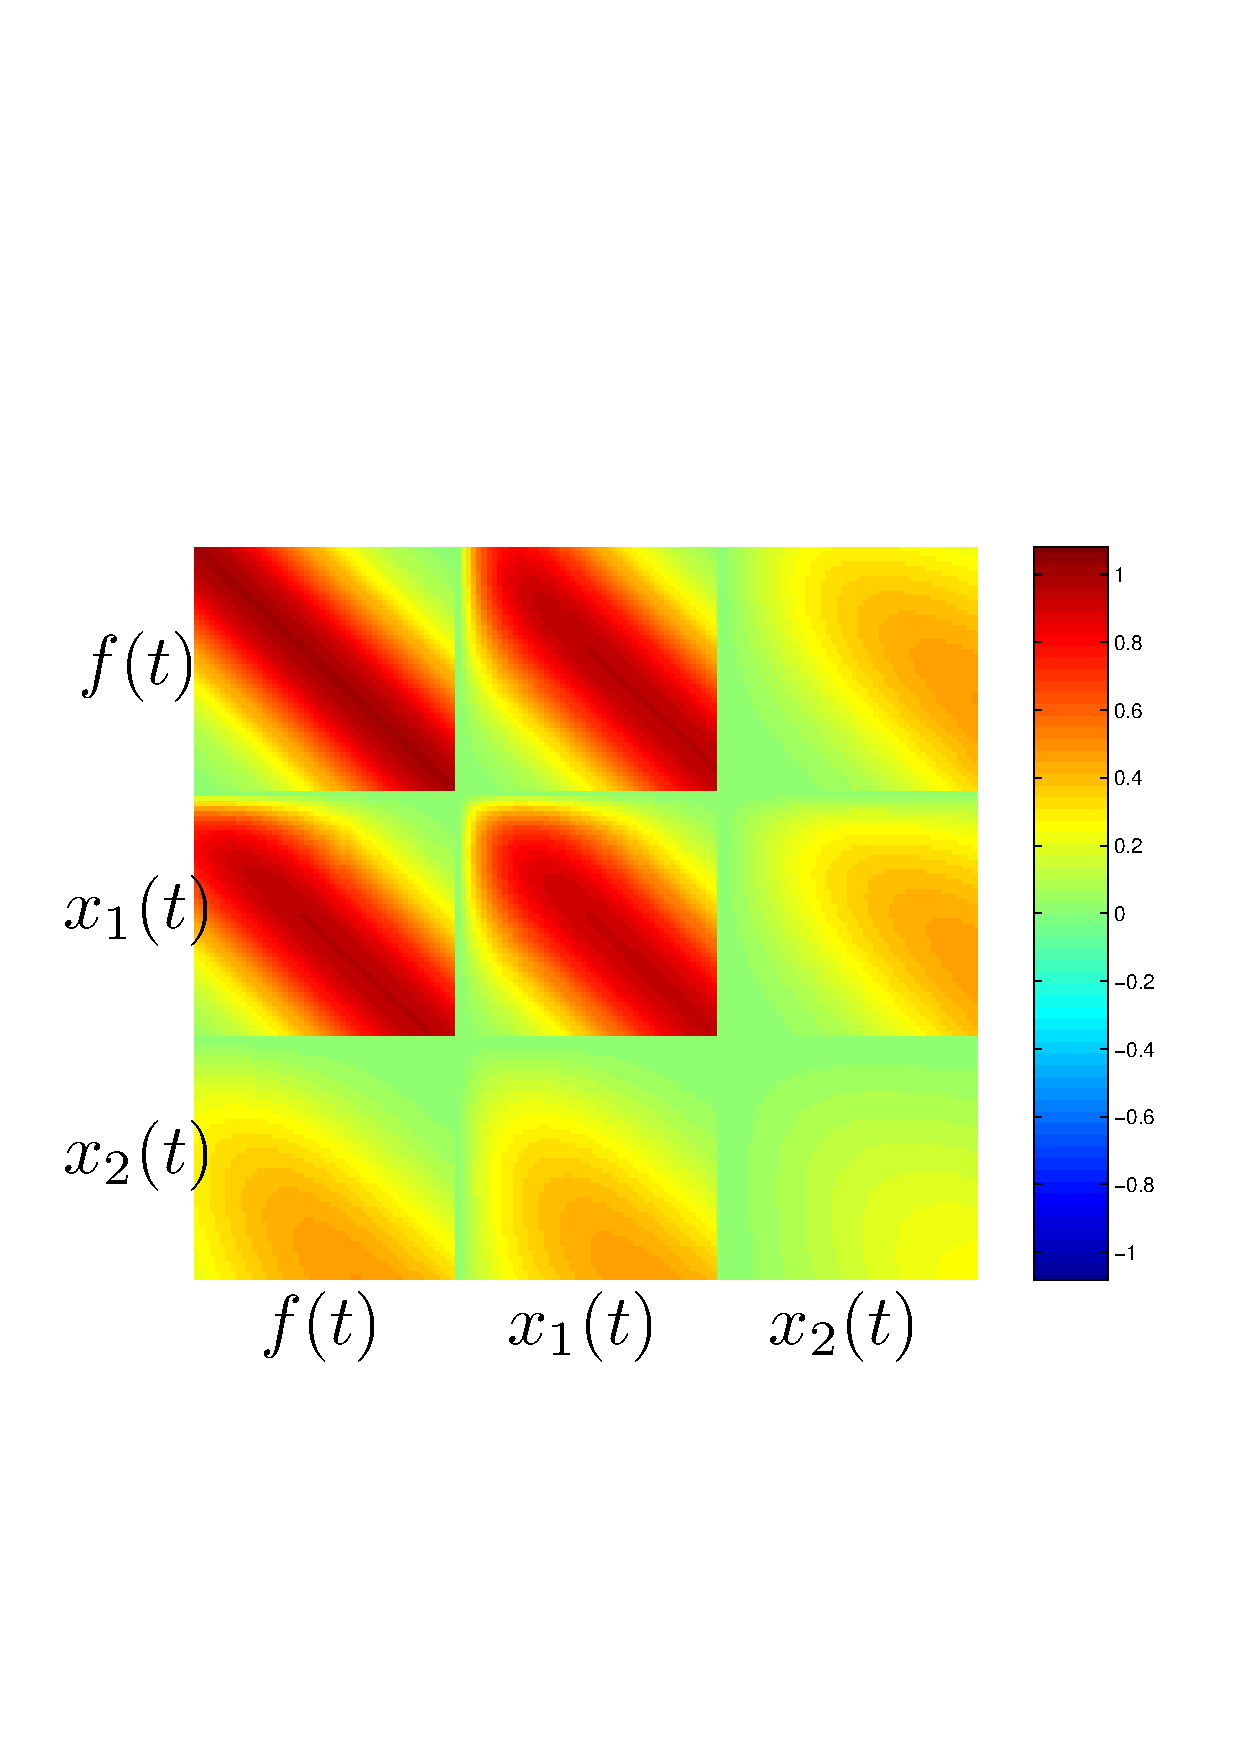
\includegraphics[width=0.8\columnwidth]{./diagrams/gpsimTestKernelImage}
% \par\end{center}

% \end{centercolumns}%{}
% %\begin{flushright}
% %\hyperlink{skipSIMSamples}{\beamergotobutton{Skip SIM Samples}}
% %\par\end{flushright}


% \lyxframeend{}\lyxframe{Prediction of the transcription factor concentration $f(t)$}

% Under the linear model, we have \begin{eqnarray*}
% \left[\begin{array}{c}
% f\\
% \mathbf{x}\end{array}\right] & \thicksim & \mathcal{N}\left(\left[\begin{array}{c}
% 0\\
% \frac{\mathbf{B}}{\mathbf{D}}\end{array}\right],\left[\begin{array}{cc}
% K_{ff} & K_{f\mathbf{x}}\\
% K_{\mathbf{x}f} & K_{\mathbf{xx}}\end{array}\right]\right)\end{eqnarray*}
%  Standard GP Regression yields the mean and covariance function of
% the predicted process as \begin{eqnarray*}
% \left\langle f\right\rangle _{post} & = & K_{f\mathbf{x}}K_{\mathbf{xx}}^{-1}\left(\mathbf{x}-\frac{\mathbf{B}}{\mathbf{D}}\right)\\
% K_{ff}^{post} & = & K_{ff}-K_{f\mathbf{x}}K_{\mathbf{xx}}^{-1}K_{\mathbf{x}f}\end{eqnarray*}



% \lyxframeend{}\subsection{Parameter Estimation}


% \lyxframeend{}\lyxframe{ Parameter Estimation for the Linear Model}

% A likelihood function for the model parameters $\theta=\{B_{j},\, S_{j},\, D_{j}\}_{j=1}^{N}$
% and GP length scale $l$ is obtained by \emph{integrating out} the
% latent function $f(t)$ \[
% L(\theta,l)=\int\left(\prod_{j}p(x_{j}|\theta,f(t))\right)p(f(t)|l)\,\mathrm{d}f(t)\]
%  Under the GP model, the log marginal likelihood is then given by
% \[
% \mathrm{log}L(\theta,l)=-\frac{1}{2}x^{T}\left(K+\sigma_{n}^{2}\mathtt{I}\right)^{-1}x-\frac{1}{2}\mathrm{log}\left\vert K+\sigma_{n}^{2}\mathtt{I}\right\vert -\frac{n}{2}\mathrm{log}2\pi\]


% Maximise to find model parameters.


% \lyxframeend{}\section{Cascaded Differential Equations}


% \lyxframeend{}\lyxframe{Outline }

% \tableofcontents{}[currentsection,hideallsubsections] 


% % \lyxframeend{}\lyxframe{Cascaded Differential Equations}

% % %\begin{flushright}
% % %\textbf{Antti Honkela}
% % %\par\end{flushright}

% % \begin{itemize}
% % \item Transcription factor protein also has governing mRNA.
% % \item This mRNA can be measured.
% % \item In signalling systems this measurement can be misleading because it
% % is activated (phosphorylated) transcription factor that counts.
% % \item In development phosphorylation plays less of a role.
% % \end{itemize}

% % \lyxframeend{}\lyxframe{Drosophila \emph{Mesoderm} Development}

% % \textbf{Data from Furlong Lab in EMBL Heidelberg.}

% % \begin{itemize}
% % \item Describe mesoderm development.
% % \end{itemize}

% \lyxframeend{}\lyxframe{Cascaded Differential Equations }

% %\begin{flushright}
% %\textbf{Antti Honkela}
% %\par\end{flushright}

% We take the production rate of active transcription factor to be given
% by \begin{align*}
% \frac{\mathrm{d}f\left(t\right)}{\mathrm{d}t} & =\sigma y\left(t\right)-\delta f\left(t\right)\\
% \frac{\mathrm{d}x_{j}\left(t\right)}{\mathrm{d}t} & =B_{j}+S_{j}f\left(t\right)-D_{j}x_{j}\left(t\right)\end{align*}
%  The solution for $f(t)$, setting transient terms to zero, is \[
% f(t)=\sigma\exp\left(-\delta t\right)\int_{0}^{t}y(u)\exp\left(\delta u\right)\mathrm{d}u\ .\]

% \lyxframeend{}


\section{Transcription Factor Target Ranking}

\frame{
  \frametitle{Outline}

  \tableofcontents[currentsection,hideallsubsections]{}
}

\frame{
  \frametitle{Target ranking: motivation}

  \begin{itemize}
  \item Finding target genes of TFs is an obvious first step in
    reverse engineering gene regulatory networks
  \item Typical techniques
    \begin{itemize}
    \item Measure TF binding locations in the genome using ChIP-chip/-seq
    \item Observe gene expression in mutants with the TF disabled
      (knockouts) or overexpressed
    \end{itemize}
  \item Endless potential applications in understanding disease and
    other biological phenomena
  \end{itemize}
}

\frame{
  \frametitle{Case study: Mesoderm and muscle development in Drosophila}

  \begin{itemize}
  \item Focus on two TFs regulating mesoderm and muscle development
    in fruit fly Drosophila: Twist and Mef2
  \item Assume no post-translational regulation of these TFs
  \item Expression data: 12 time points at 1 h intervals, 3 replicates
  \item Data averaged over the whole embryo
  \end{itemize}
}

\setbeamercovered{invisible}

\frame{
  \frametitle{Application of the models to target ranking}

  \begin{itemize}
  \item First apply the two-layer model for each target gene
    independently
  \item Ranking by marginal likelihood
  \end{itemize}

  \setbeamercovered{invisible}
  \pause
  \begin{figure}
    \flushleft
    \includegraphics[width=.4\textwidth]{diagrams/twi_FBgn0040600.png}
    \hspace*{-23mm}
    \includegraphics<3->[width=.4\textwidth]{diagrams/twi_FBgn0000927.png}
    \hspace*{-23mm}
    \includegraphics<4->[width=.4\textwidth]{diagrams/twi_FBgn0011206.png}
    \hspace*{-23mm}
    \includegraphics<5>[width=.4\textwidth]{diagrams/twi_FBgn0039286.png}
    \caption{Fitted two-layer (GPDISIM) models}
  \end{figure}
}


\frame{
  \frametitle{Application of the models to target ranking}

  \begin{itemize}
  \item Need to exclude inactive genes: compare to a model with
    $S=0$
    \begin{itemize}
    \item (``Normalised score'': rank by difference of log-likelihoods)
    \item ``Filtered score'': filter by difference, rank by score
    \end{itemize}
  \item Using a set of identified likely targets as a training set,
    learn multiple-target models for training set + each target
    individually
  \end{itemize}

%   \pause
%   \begin{figure}
%     \flushleft
%     \includegraphics[width=.4\textwidth]{diagrams/twi_gpsim_example3}
%     \hspace*{6mm}
%     \includegraphics<3>[width=.4\textwidth]{diagrams/twi_gpsim_example4}
%     \caption{Fitted single-layer (GPSIM) models}
%   \end{figure}
}

\subsection{Target ranking results}

\frame{
  \frametitle{Evaluation methods}

  \begin{itemize}
  \item Evaluate the ranking methods by taking a number of top-ranked
    targets and record the number of
    ``positives''~\citep{Zinzen2009,Sandmann06,Sandmann07}:
    \begin{itemize}
    \item targets differentially expressed in TF knock-outs
    \item targets with ChIP-chip binding sites within 5 kb of gene
    \end{itemize}
  \item Compare against
    \begin{itemize}
    \item Ranking by correlation of expression profiles
    \item Ranking by $q$-value of differential expression
      in knock-outs
    \end{itemize}
  \item Optionally focus on genes with annotated expression in
    tissues of interest
  \end{itemize}
}

\frame{
  \frametitle{Results}

  \begin{center}
    \includegraphics[width=\textwidth,trim=0mm 3mm 0mm 0mm]{diagrams/dros_comparison_for_slides_2010-05-07} \\
    {\tiny '***': $p < 0.001$, '**': $p < 0.01$, '*': $p < 0.05$}
  \end{center}
}


\section{Non-linear multiple-TF models}

\frame{
  \frametitle{Extending the model}

  \begin{itemize}
  \item The linear single-TF model is about as far as exact inference
    takes us
  \item More complicated models require approximate techniques
    (e.g.\ MCMC)
  \item With MCMC there are no restrictions on the functional forms of
    models used
  \end{itemize}
}

\frame{
  \frametitle{The full model}

  \begin{itemize}
  \item Consider the ODE transcription regulation model for multiple
    TFs
    $$
    \frac{d x_j (t)} {d t} =
    B_j + S_j g(f_1(t),\ldots,f_I(t); \bfw_j) - D_j x_j(t)
    $$
  \item $g(\cdot )$ a positive \textcolor{blue}{sigmoidal activation function}
  \item $\bfw_j$ \textcolor{blue}{interaction weights} between the $j$th
    gene and the set of $I$ TFs
  \end{itemize}
}

\frame
{

\frametitle{Gene regulation with multiple TFs} 

$$
\frac{d x_j (t)} {d t} =
B_j + S_j g(f_1(t),\ldots,f_I(t); \bfw_j) - D_j x_j(t),
$$

\begin{itemize}
\item $g(\cdot)$ is assumed to 
     be a \textcolor{blue}{multiple-TF hill function}:
$$
g(f_1(t),\ldots,f_I(t); \bfw_j)
= \frac{\prod_{i=1}^I f_i(t)^{w_{ji}}}
{\gamma_j^{\sum_{i=1}^I w_{ji}} + \prod_{i=1}^I f_i(t)^{w_{ji}}} 
$$
where $w_{ji}$ can be both positive and negative 

\item The above can also be written as the \textcolor{blue}{sigmoid function}: 

$$
g(f_1(t),\ldots,f_I(t); \bfw_j)
= \frac{1}{1 + e^{-w_{j0}  - \sum_{i=1}^I w_{ji} \log f_i(t)}}
$$
where we defined  $w_{j0} = - \sum_{i=1}^I w_{ji} \log \gamma_j$ 
as new parameter 

\end{itemize}
}


\frame{
  \frametitle{Bayesian inference from mRNA data: priors}


$$
x_j(t) = \frac{B_j}{D_j} +  \left(A_j - \frac{B_j}{D_j}\right) e^{-D_j t} +
S_j \int_{0}^t g(f_i(u),\ldots,f_I(u); \bfw_j) e^{-D_j(t- u)} du 
$$

$$
f_i (t) = \int_0^t m^f_i (t) e^{- d_i (t-u)} d u
$$

\begin{itemize}

\item We place priors on: 

    \begin{itemize}
   
    \item \textcolor{blue}{Kinetics:} $\Theta = \{A_j,B_j,D_j,S_j\}_{j=1}^N$ (uniform or
          log normal) 
        
     \item \textcolor{blue}{Decays} of TF mRNA: $\{d_i\}$, (uniform or log normal)   

     \item \textcolor{blue}{Interaction} weights: $\{\bfw_j\}$, 
           (Gaussian priors with optionally positivity constraints
           and/or spike and slab sparse priors) 

     \item \textcolor{blue}{mRNA functions} $m_i^f(t)$: \textcolor{red}{Gaussian processes}
           (through a transformation that ensures positivity of $m_i^f(t)$) 

     \item \textcolor{blue}{Lengthscales} of Gaussian processes (uniform or gamma) and 
            \textcolor{blue}{noise variances} in the likelihoods (gamma)  

\end{itemize}

\end{itemize}

}



\frame{
  \frametitle{Bayesian inference from mRNA data: MCMC} 


$$
\text{joint} 
= p(\widetilde{X}|X) p(\widetilde{M}^f|M^f) p(\bar{M}_i^f) p(\Theta) 
 p(W) p(\{d_i\}_{i=1}^I) p(\{\sigma_j^2\}) p(\{\ell^2\}_{i=1}^I)
$$


\begin{itemize}

\item \textcolor{blue}{Many Metropolis-Hastings} steps involving sampling Gaussian process
      functions, kinetic parameters, interaction weights, etc.  


\item We can afford training the model using MCMC 
      in \textcolor{blue}{moderate-sized} networks,
      e.g.\ with 100 genes and 5 TFs and 3 replicas, 
      \textcolor{blue}{but not genome-wide} (too slow for that)  


\item But once the model in trained, \textcolor{blue}{we can do 
      genome-wide} prediction (e.g.\ gene \textcolor{blue}{target identification})
      and this is fast 

\end{itemize}
}


\frame
{

\frametitle{Experiments in Drosophila data} 



\begin{itemize}

\item Microarray dataset containing three replicas of $12$ time points collected hourly throughout
Drosophila embryogenesis in wild-type embryos 

\item \textcolor{blue}{$92$ target genes} 

\item  \textcolor{blue}{$5$ TFs} (including 
        \textcolor{blue}{Twist and Mef2} which regulate mesoderm and muscle development)


\item ChiP information is used to define the (deterministic) sparse
  prior one interaction between TFs and target genes  


\end{itemize}
}


\frame{
  \frametitle{Experiments in Drosophila data} 


  \includegraphics<1>[width=100mm,height=70mm]{masamb/DrosTrain925TfsProfiles.pdf}
  \includegraphics<2>[width=100mm,height=70mm]{masamb/DrosTrain925TfsmRNATFs.pdf}
  \includegraphics<3>[width=100mm,height=70mm]{masamb/DrosTrain925TfsGenes1.pdf}
  \includegraphics<4>[width=100mm,height=70mm]{masamb/DrosTrain925TfsGenes2.pdf}
  \includegraphics<5>[width=100mm,height=70mm]{masamb/DrosTrain925TfsGenes3.pdf}
}

\frame
{
\frametitle{Genome-wide gene ranking/identification}

\begin{itemize}

\item Assume that we have trained our model in a carefully chosen 
  set of genes. This gives the \textcolor{blue}{posterior distribution of TF profiles} 


 \item Given a test (unknown gene), called $*$, can we use the trained
   model to make (probabilistic) \textcolor{blue}{statements about if a certain 
   TF  regulates $*$?}  

  
 \item We need to compute \textcolor{blue}{Bayesian prediction probabilities}  

\end{itemize}


}


\frame
{
\frametitle{Genome-wide gene ranking/identification}


\begin{itemize}

\item Let $\bar{\bfy}_*$ be a finite set of noisy observations of the 
      test gene mRNA function $y_*(t)$ where

\end{itemize}
   
$$
y_*(t) = \frac{B_*}{D_*} +  \left(A_* - \frac{B_*}{D_*}\right) e^{-D_* t} +
S_* \int_{0}^t g(f_i(u),\ldots,f_I(u); \bfw_*) e^{-D_*(t- u)} du, 
$$




where now the  \textcolor{blue}{new prior} over TFs (function
$f_i(\cdot),\ldots,f_I(\cdot)$) is the \textcolor{blue}{Bayesian posterior} 
$p(f_i(\cdot),\ldots,f_I(\cdot)| \widetilde{Y}, \widetilde{M}^f)$
obtained previously. 


\begin{itemize}

 
\item We wish to compute the posterior probability of the event
      \textcolor{red}{"$i$th  TF regulates gene *"}
    



\item We can similarly define events involving more that two TFs 

\end{itemize}


}










\frame
{

\frametitle{Genome-wide gene ranking/identification}


\begin{itemize}

\item "$i$th TF regulates gene *" \textcolor{blue}{$\Longleftrightarrow$} 
   ``the interaction $w_{*i}$ is zero or not'' 

\item We need to search over all possible models where some interactions are
set to zero. Two ways:  

\begin{enumerate}

\item Define all models $\mathcal{M}_1, \mathcal{M}_2, \ldots$ 
      obtained by \textcolor{blue}{switching on/off TFs}. For $I$ 
      TFs we have $2^I$ possible models 


\item Use a single large model with a \textcolor{blue}{sparse prior} over the 
      \textcolor{blue}{interaction} weights $\bfw_*$ 
       


\end{enumerate}

\end{itemize}

\textcolor{red}{\bf Remark:}\textcolor{red}{ 
1) is more convenient when $I$ is small (say less than $5$), while 2) more
tractable for larger $I$} 
 

}




\frame
{

\frametitle{Genome-wide gene ranking/identification}


$$
p(i \text{TF present}|\bfy_*, Y,  \widetilde{M}^f)
\propto \sum_{\mathcal{M}_k : w_{*i} \neq 0 } p(\bfy_*| \bar{Y},
  \widetilde{M}^f, \mathcal{M}_k) p(\mathcal{M}_k)
$$

This requires computing the \textcolor{blue}{predictive density} for each 
model $\mathcal{M}_k$ 

\begin{multline}
p(\bfy_*| \bar{Y},
\widetilde{M}^f, \mathcal{M}_k) = \\ 
\int_{\bfw_*,\bftheta_*,\{f_i\}} p(\bfy_* | \bfw_*,\bftheta_*,\{f_i\}_{i=1}^I, \mathcal{M}_k) 
p(\bfw_*) p(\bftheta_*) p(\{f_i\}_{i=1}^I | \bar{Y},
  \widetilde{M}^f) \nonumber 
\end{multline}
where $\bftheta_* = (B_*,D_*,S_*,A_*)$ and the posterior  
$p(\{f_i\}_{i=1}^I | \bar{Y}, \widetilde{M}^f)$ over TFs has been 
obtained in the training phase.  


}




\frame
{

\frametitle{Genome-wide gene ranking/identification}


Using the samples drawn from the posterior $p(\{f_i\}_{i=1}^I |
\bar{Y}, \bar{M}^f)$:
\begin{multline}
p(\bfy_*| \bar{Y},
\widetilde{M}^f, \mathcal{M}_k) \approx \\ 
 \int_{\bfw_*,\bftheta_*} \left(
\frac{1}{T}\sum_{t=1}^T  p(\bfy_* |
\bfw_*,\bftheta_*,\{f^{(t)}_i\}_{i=1}^I, \mathcal{M}_k) 
\right) p(\bfw_*) p(\bftheta_*) \nonumber 
\end{multline}
We approximate this predictive 
density  by drawing samples 
from $p(\bfw_*,\bftheta_*|\bfy_*,\bar{Y},\bar{M}^f)$
and then using Chib's (1995) approximation to a marginal likelihood:

$$
p(\bfy_*) = \frac{q(\bfy_* | \bfw_*^s, \bftheta_*^s ) p(\bfw_*^s)
  p(\bftheta_*^s)}{q(\bfw_*^s,\bftheta^s_*|\bfy_*)} 
$$
where $(\bfw_*^s,\bftheta^s_*)$ are certain values, 
and $q(\bfw_*^s,\bftheta^s_*|\bfy_*)$ is a density estimator of the true 
posterior  $p(\bfw_*^s,\bftheta^s_*|\bfy_*)$



}



\frame
{

\frametitle{Genome-wide gene ranking/identification}


\begin{itemize}

\item The above procedure is \textcolor{blue}{very fast}: it takes 1/2 mins for each gene.  


\item The key to achieve such speed to is to use the \textcolor{blue}{data augmentation principle} 
when sampling $p(\bfw_*,\bftheta_*|\bfy_*,\bar{Y},\bar{M}^f)$  using
MCMC (i.e.\ sample also the TFs $\{f_i\}$ from the ``cached'' samples)

\end{itemize}

\textcolor{red}{\bf Remark}: \textcolor{red}{Speed is important because we
  need to repeat such a procedure for any test gene in order to do genome-wide target identification}

}

\section{Experimental structure of time series assays}


\frame{
  \frametitle{Molecular biology time series}

  \begin{itemize}
  \item Biological systems are dynamic, observing their time evolution
    very helpful
  \item Time series measurements of gene expression, protein activity,
    protein binding, ...
  \item Problem: most of these assays are highly disruptive to the
    sample
  \item Therefore: time series = series of independent experiments
    run for different lengths of time
  \item This has implications for modelling...
  \end{itemize}
}

\section{The data}

\frame{
  \frametitle{Outline}

  \tableofcontents
}

\frame{
  \frametitle{Outline}

  \tableofcontents[currentsection]{}
}

\frame{
  \frametitle{Simulated molecular biology time series}

  \begin{center}
    \includegraphics<1>[width=.65\textwidth]{figures/crosssec_example_1_1}
    \includegraphics<2>[width=.65\textwidth]{figures/crosssec_example_2_1}
    \includegraphics<3>[width=.65\textwidth]{figures/crosssec_example_3_1}
    \includegraphics<4>[width=.65\textwidth]{figures/crosssec_example_4_1}
    \includegraphics<5>[width=.65\textwidth]{figures/crosssec_example_1_2}
    \includegraphics<6>[width=.65\textwidth]{figures/crosssec_example_2_2}
    \includegraphics<7>[width=.65\textwidth]{figures/crosssec_example_3_2}
    \includegraphics<8>[width=.65\textwidth]{figures/crosssec_example_4_2}
    \includegraphics<9>[width=.65\textwidth]{figures/crosssec_example_1_3}
    \includegraphics<10>[width=.65\textwidth]{figures/crosssec_example_2_3}
    \includegraphics<11>[width=.65\textwidth]{figures/crosssec_example_3_3}
    \includegraphics<12>[width=.65\textwidth]{figures/crosssec_example_4_3}
  \end{center}
}

\frame{
  \frametitle{Real gene expression time series}

  \begin{center}
    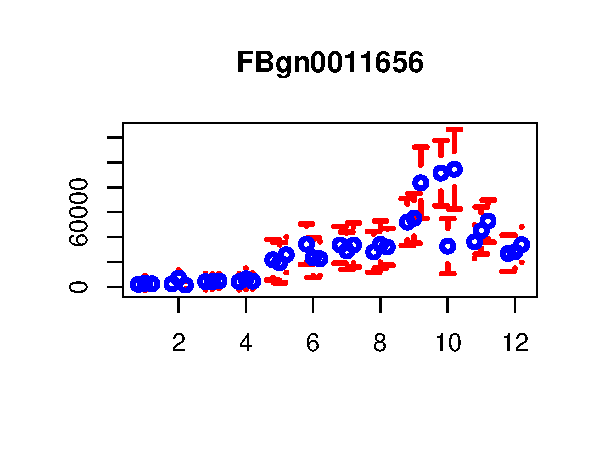
\includegraphics[width=.33\textwidth,trim=9mm 9mm 9mm 9mm]{figures/dros_expression_series_1}
    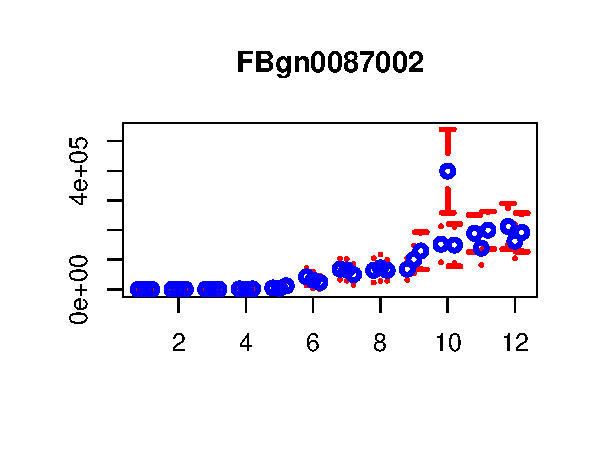
\includegraphics[width=.33\textwidth,trim=9mm 9mm 9mm 9mm]{figures/dros_expression_series_5}
    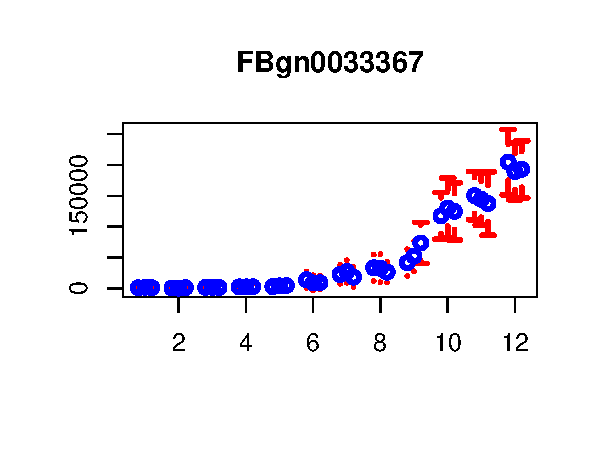
\includegraphics[width=.33\textwidth,trim=9mm 9mm 9mm 9mm]{figures/dros_expression_series_3}\\
    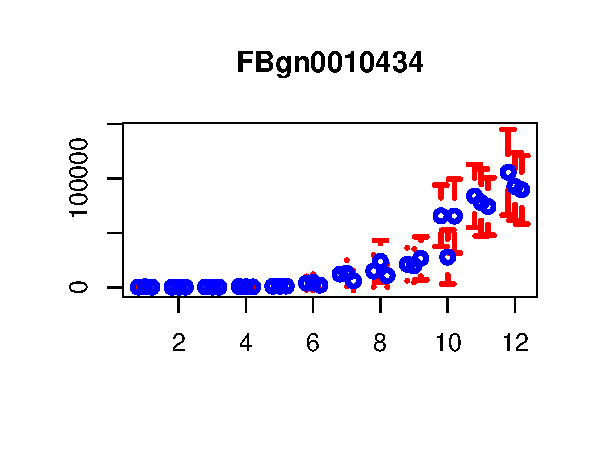
\includegraphics[width=.33\textwidth,trim=9mm 9mm 9mm 9mm]{figures/dros_expression_series_4}
    %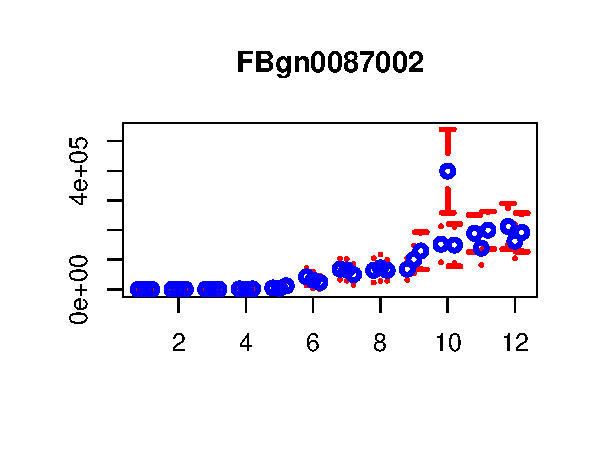
\includegraphics[width=.33\textwidth,trim=9mm 9mm 9mm 9mm]{figures/dros_expression_series_5}
    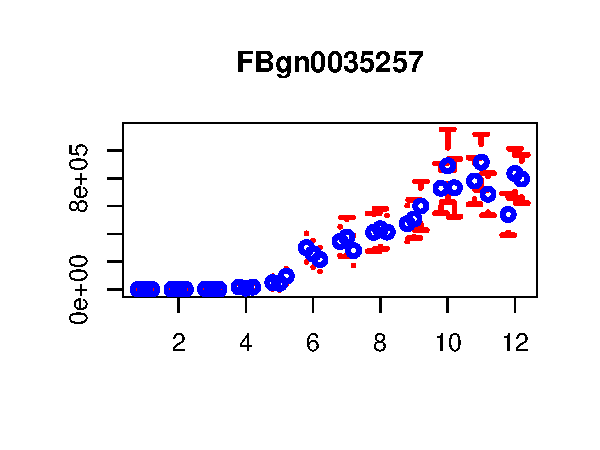
\includegraphics[width=.33\textwidth,trim=9mm 9mm 9mm 9mm]{figures/dros_expression_series_6}
    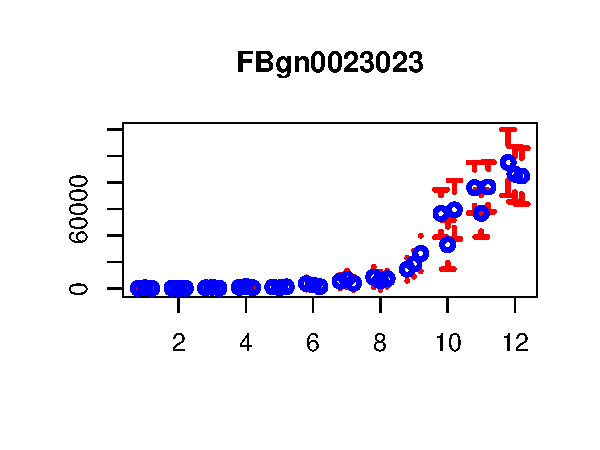
\includegraphics[width=.33\textwidth,trim=9mm 9mm 9mm 9mm]{figures/dros_expression_series_7}\\
    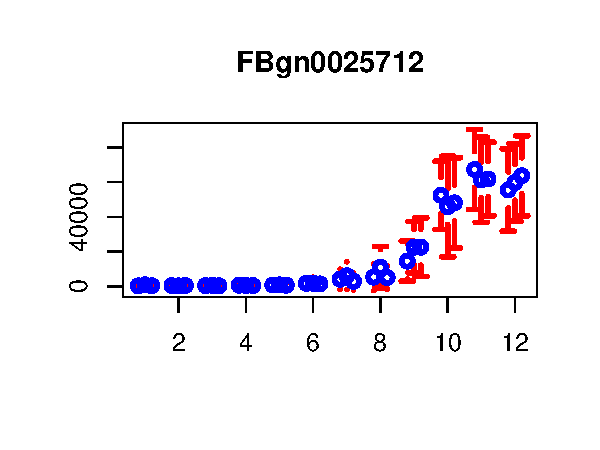
\includegraphics[width=.33\textwidth,trim=9mm 9mm 9mm 9mm]{figures/dros_expression_series_8}
    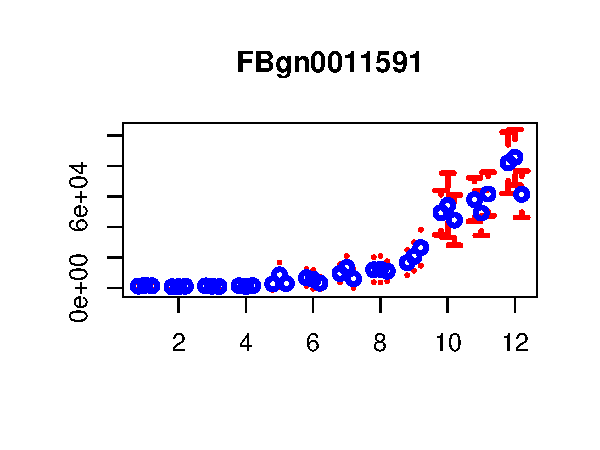
\includegraphics[width=.33\textwidth,trim=9mm 9mm 9mm 9mm]{figures/dros_expression_series_10}
    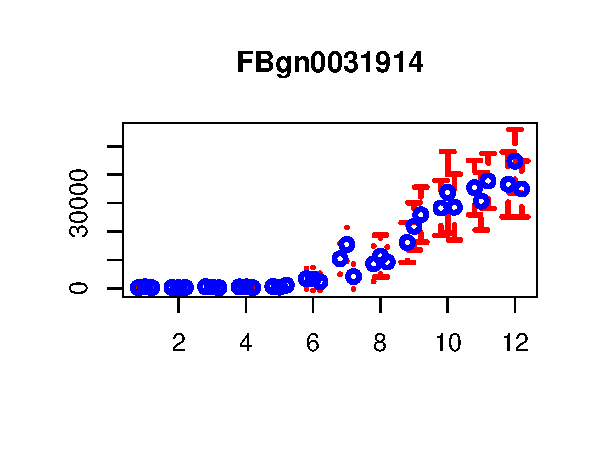
\includegraphics[width=.33\textwidth,trim=9mm 9mm 9mm 9mm]{figures/dros_expression_series_11}
  \end{center}
}

\section{Models: theory}

\frame{
  \frametitle{Outline}

  \tableofcontents[currentsection]{}
}

\frame{
  \frametitle{Example model: Linear ODE model of transcription}

  \begin{itemize}
  \item Linear Activation Model (\citealp{Barenco:ranked06}, Genome
    Biology) \[
    \frac{\mymathrm{d}x_{j}\left(t\right)}{\mymathrm{d}t}=B_{j}+S_{j}f\left(t\right)-D_{j}x_{j}\left(t\right)\]
 
  \item $x_{j}(t)$ -- concentration of gene $j$'s mRNA 
  \item $f(t)$ -- concentration of active transcription factor 
  \item Model parameters: baseline $B_{j}$, sensitivity $S_{j}$ and
    decay $D_{j}$ 
  \item Placing a Gaussian process (GP) prior on $f(t)$ leads to
    a joint GP over all concentration profiles (\citealp{Gao08ECCB},
    Bioinformatics)
  \end{itemize}
}

\frame{
  \frametitle{How to connect the model to data?}

  \begin{enumerate}
  \item Assume \myred{independent profiles} for each complete
    (biological) repeat
    \begin{itemize}
    \item Loses statistical power for extra independence assumptions
    \item Is it meaningful to order the repeats?
    \end{itemize}
  \item Assume one \myred{shared underlying profile} with independent
    observations
    \begin{itemize}
    \item Potentially sensitive to outliers
    \end{itemize}
  \end{enumerate}
}

\frame{
  \frametitle{Exchangeability analysis}

  Assume $x_j^k(t_i)$ observation of $k$th repeat of $j$th gene at $i$th time

  \begin{tabular}{lcc}
    & $x_:^k(t_i) \leftrightarrow x_:^{k'}(t_i)$ & $x_j^k(t_i) \leftrightarrow x_j^{k'}(t_i)$ \\
    & ``swap arrays'' & ``swap single gene'' \\
    \hline
    ``Reality'' & \mygreen{Yes} & \mygreen{No} \\
    1. Independent profiles & \myred{No} & \mygreen{No} \\
    2. Shared profile & \mygreen{Yes} & \myred{Yes} \\
  \end{tabular}
}

\frame{
  \frametitle{Solution: hierarchical GP model}

  \begin{itemize}
  \item Assume the underlying $f(t)$ is composed of a shared and an
    experiment-specific part $f_{ik}(t)$
\[
    \frac{\mymathrm{d}x_{j}\left(t\right)}{\mymathrm{d}t}=B_{j}+S_{j}[f_{\text{shared}}\left(t\right) + f_{ik}\left(t\right)]-D_{j}x_{j}\left(t\right)
    \]
  \item Covariance is of the same form as usual
  \item Introduces additional covariance terms for measurements from
    the same experiment
  \item Alternative parametrisations of variance of $f_{ik}(t)$
    \begin{itemize}
    \item Shared across all experiments
    \item Sampled independently for each experiment
    \end{itemize}
  \end{itemize}
}

\frame{
  \frametitle{Exchangeability analysis revisited}

  Assume $x_j^k(t_i)$ observation of $k$th repeat of $j$th gene at $i$th time

  \begin{tabular}{lcc}
    & $x_:^k(t_i) \leftrightarrow x_:^{k'}(t_i)$ & $x_j^k(t_i) \leftrightarrow x_j^{k'}(t_i)$ \\
    & ``swap arrays'' & ``swap single gene'' \\
    \hline
    ``Reality'' & \mygreen{Yes} & \mygreen{No} \\
    1. Independent profiles & \myred{No} & \mygreen{No} \\
    2. Shared profile & \mygreen{Yes} & \myred{Yes} \\
    3. Hierarchical model & \mygreen{Yes} & \mygreen{No} \\
  \end{tabular}
%   \begin{tabular}{lccc}
%     & Indep.\ profiles & Shared profile & Hierarchical \\
%     $x_:^k(t_i) \leftrightarrow x_:^{k'}(t_i)$ & \myred{No} & \mygreen{Yes} & \mygreen{Yes} \\
%     $x_j^k(t_i) \leftrightarrow x_j^{k'}(t_i)$ & \mygreen{No} & \myred{Yes} & \mygreen{No} \\
%   \end{tabular}
}

\section{Models: practice}

\frame{
  \frametitle{Outline}

  \tableofcontents[currentsection]{}
}

\frame{
  \frametitle{ODE model of translation and transcription}

  \begin{itemize}
  \item Assume TF is transcriptionally regulated with related mRNA
    $y(t)$
  \item This yields a system of ODEs \citep{Gao08ECCB}
    \begin{align*}
      \frac{\mymathrm{d}f\left(t\right)}{\mymathrm{d}t} & =\sigma y\left(t\right)-\delta f\left(t\right)\\
      \frac{\mymathrm{d}x_{j}\left(t\right)}{\mymathrm{d}t} & =B_{j}+S_{j}f\left(t\right)-D_{j}x_{j}\left(t\right)
    \end{align*}
  \item The corresponding GP model can be derived analogously to the
    previous case
  \end{itemize}
}

\frame{
  \frametitle{Independent profiles}

  \begin{center}
    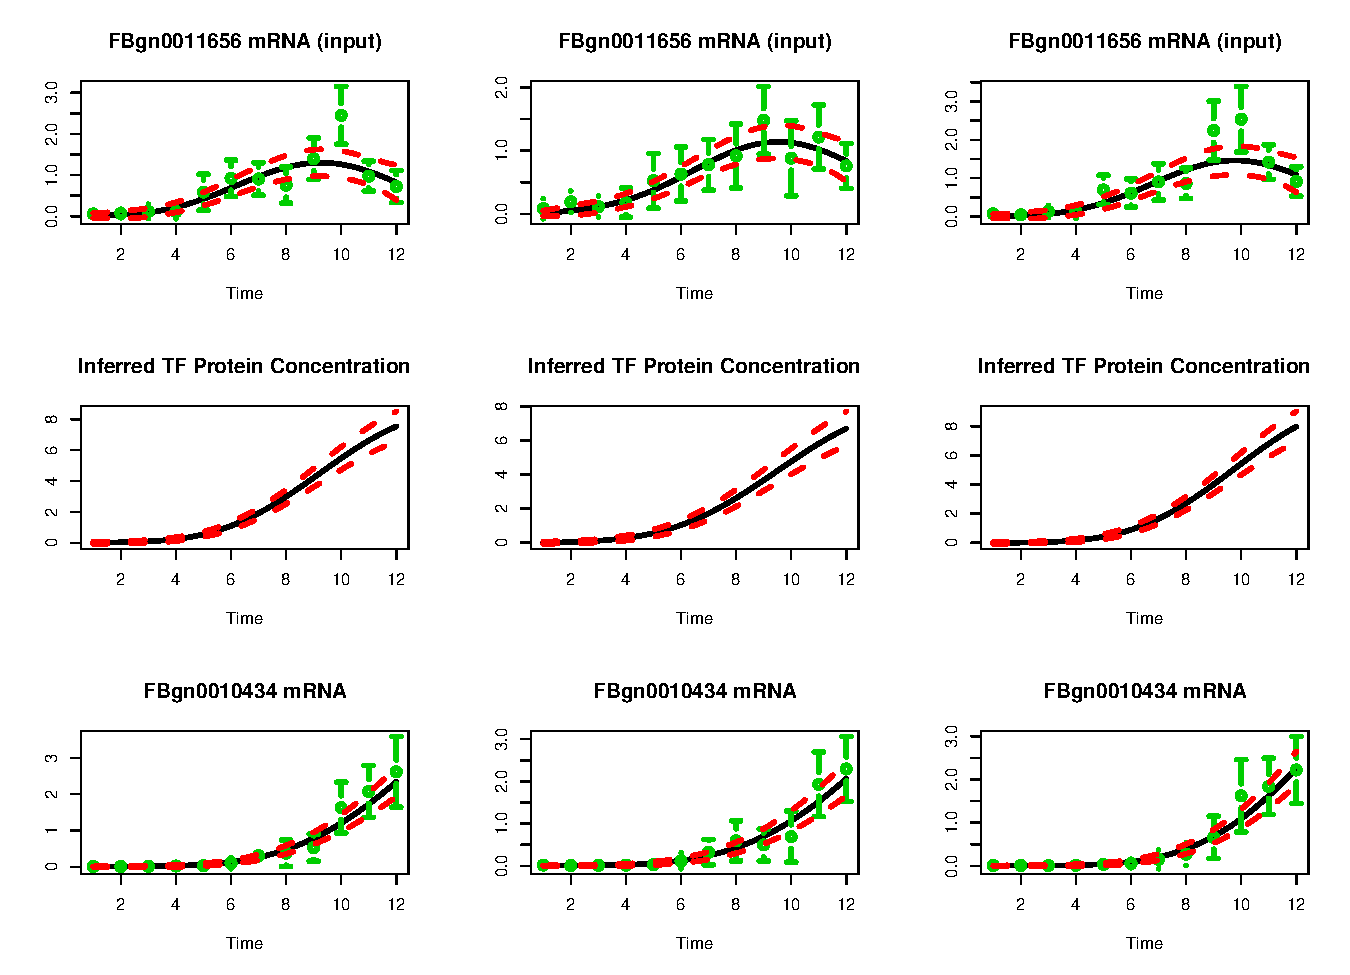
\includegraphics[scale=0.45]{figures/old_sample_model}
  \end{center}
}

\frame{
  \frametitle{Hierarchical model}

  \begin{center}
    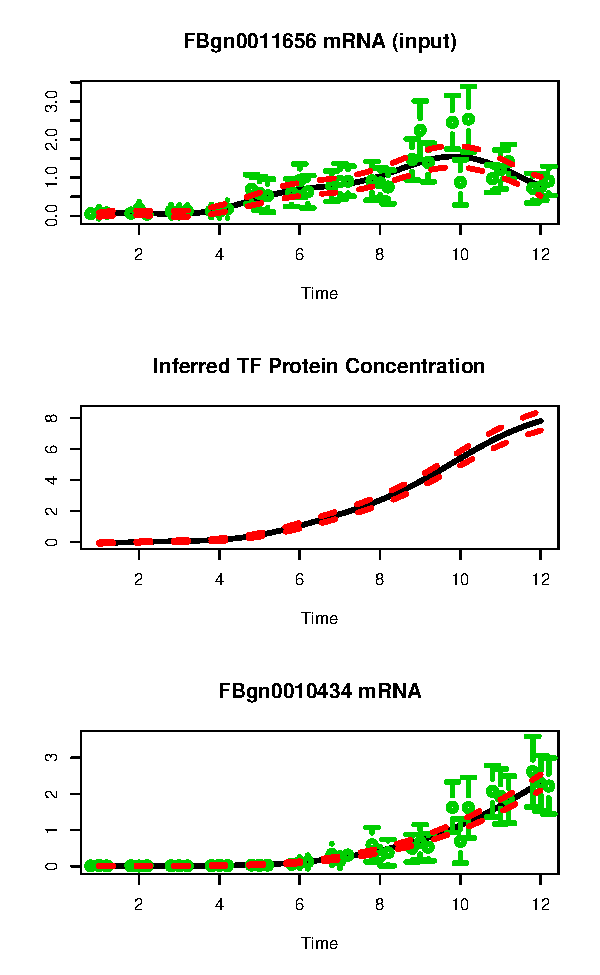
\includegraphics[scale=0.5]{figures/hier_sample_model}
  \end{center}
}

\section{Conclusion}

% \frame{
%   \frametitle{Outline}

%   \tableofcontents[currentsection]{}
% }

\frame{
  \frametitle{Conclusion}

  \begin{itemize}
  \item Previous models of time series expression data are wrong
    \begin{itemize}
    \item Invalid exchangeability assumptions
    \end{itemize}
  \item Proposed hierarchical model rectifies this
  \item Open problems / work in progress
    \begin{itemize}
    \item Need to move beyond Gaussian likelihoods?
    \item How to do MCMC in these models?
    \end{itemize}
  \end{itemize}
}


\frame{
  \frametitle{}
}

\frame{
  \frametitle{}
}

\frame{
  \frametitle{}
}

\section{Summary}


\lyxframeend{}\lyxframe{Outline }

\tableofcontents{}[currentsection,hideallsubsections] 


\lyxframeend{}\lyxframe{Summary and Future Work}

\begin{itemize}
\item Gaussian process prior on unobserved chemical species
\item Joint Gaussian process over all observable species
  %\begin{itemize}
  %\item Efficient inference (no MCMC needed for the linear model!)
  %\end{itemize}
\item Parameter estimation by maximising the marginal likelihood
\item Ranking of candidate targets by model marginal likelihood
\item Future work (some on-going):
  \begin{itemize}
  \item Improved nonlinear models, MCMC inference
  \item Extension to multiple transcription factor models
  \item Stochastic differential equation models
  \end{itemize}
\end{itemize}


\frame{
  \frametitle{}
}


%\lyxframeend{}\lyxframe{Discussion and Future Work }

%\begin{itemize}
%\item Integration of probabilistic inference with mechanistic models.
%\item These results are small simple systems.
%\end{itemize}

% \lyxframeend{}\section{Acknowledgements}


% \lyxframeend{}\lyxframe{Outline }

% \tableofcontents{}[currentsection,hideallsubsections] 


\lyxframeend{}\lyxframe{Acknowledgements }

\begin{itemize}
\item Pei Gao, Neil Lawrence and Magnus Rattray of University of Manchester
\item Charles Girardot and Eileen Furlong of EMBL Heidelberg
%\item Martino Barenco and Mike Hubank at the Institute of Child Health in
%UCL (p53 pathway). 
% \item Raya Khanin and Ernst Wit of the University of Glasgow and the University
% of Lancaster (\emph{E. coli} repressor system). 
\end{itemize}
% {\footnotesize Funded by the BBSRC award {}``Improved Processing
% of microarray data using probabilistic models'' and EPSRC award {}``Gaussian
% Processes for Systems Identification with applications in Systems
% Biology''} \ \\
%  \ \\

\nocite{Honkela2010PNAS,Gao:latent08,GPMLBook}
%,GPMLBook,Carroll05}

\lyxframeend{}\lyxframe{References}

{\tiny \bibliographystyle{pdf_abbrvnat}
\bibliography{mpitalk}
}{\tiny \par}


\lyxframeend{}

\end{document}
